\documentclass[landscape]{article}

\usepackage{mathpazo}
\usepackage[scaled=0.9]{helvet}
\linespread{1.025}

\usepackage{geometry}
\geometry{left=2cm,right=2cm,top=2cm,bottom=2cm}

\usepackage{tikz}

\begin{document}
    \pagenumbering{gobble}
    \begin{center}
        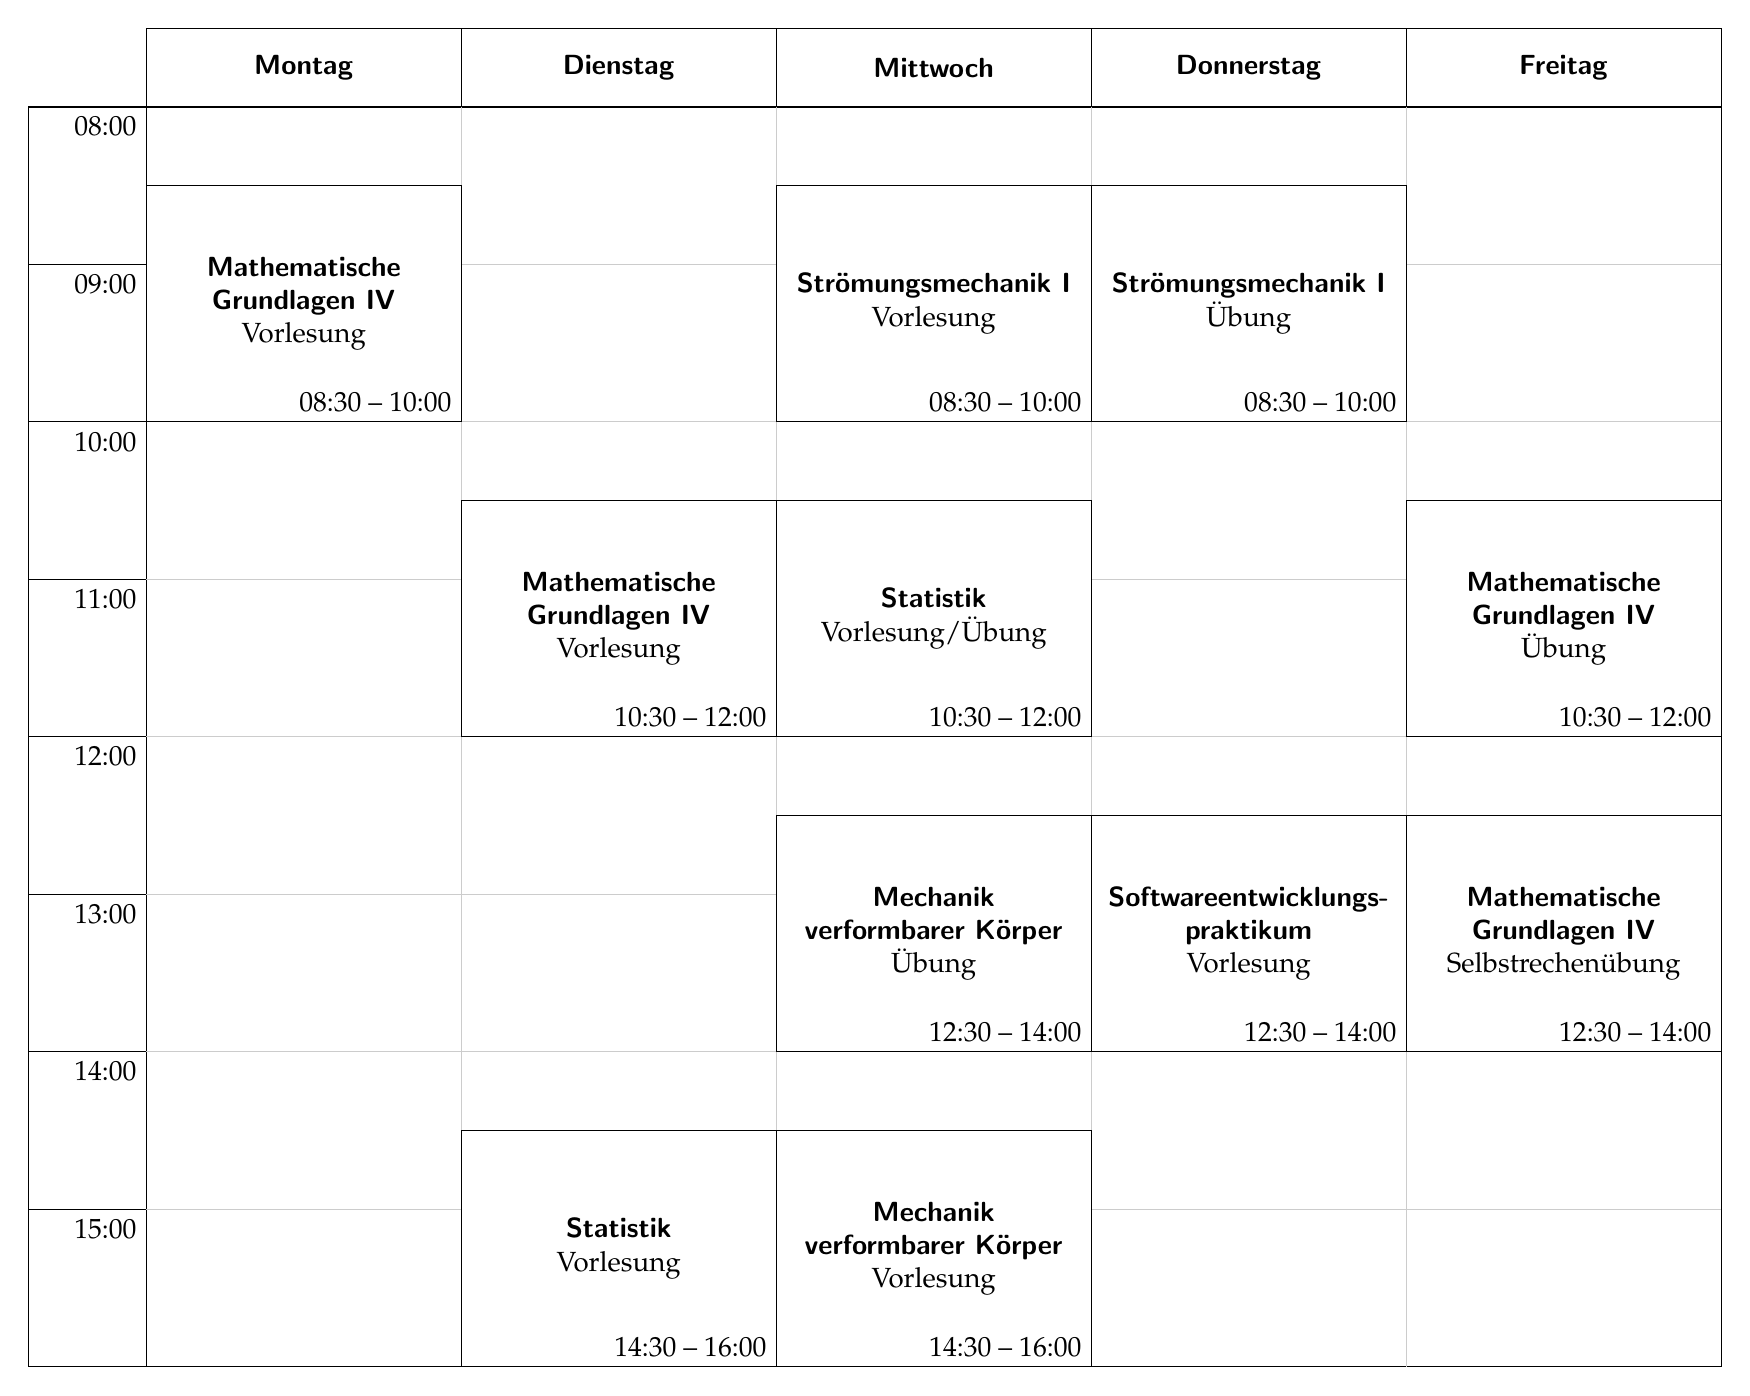
\begin{tikzpicture}
            \draw (0,-1) rectangle (1.5,-3);
            \node[anchor=north east] at (1.5,-1) {08:00};
            \draw (0,-3) rectangle (1.5,-5);
            \node[anchor=north east] at (1.5,-3) {09:00};
            \draw (0,-5) rectangle (1.5,-7);
            \node[anchor=north east] at (1.5,-5) {10:00};
            \draw (0,-7) rectangle (1.5,-9);
            \node[anchor=north east] at (1.5,-7) {11:00};
            \draw (0,-9) rectangle (1.5,-11);
            \node[anchor=north east] at (1.5,-9) {12:00};
            \draw (0,-11) rectangle (1.5,-13);
            \node[anchor=north east] at (1.5,-11) {13:00};
            \draw (0,-13) rectangle (1.5,-15);
            \node[anchor=north east] at (1.5,-13) {14:00};
            \draw (0,-15) rectangle (1.5,-17);
            \node[anchor=north east] at (1.5,-15) {15:00};
            \draw (1.5,0) rectangle (5.5,-1) node[pos=.5] {\textbf{\sffamily Montag}};
            \draw (5.5,0) rectangle (9.5,-1) node[pos=.5] {\textbf{\sffamily Dienstag}};
            \draw (9.5,0) rectangle (13.5,-1) node[pos=.5] {\textbf{\sffamily Mittwoch}};
            \draw (13.5,0) rectangle (17.5,-1) node[pos=.5] {\textbf{\sffamily Donnerstag}};
            \draw (17.5,0) rectangle (21.5,-1) node[pos=.5] {\textbf{\sffamily Freitag}};
            \draw[white!80!black] (1.5,-3) -- (21.5,-3);
            \draw[white!80!black] (1.5,-5) -- (21.5,-5);
            \draw[white!80!black] (1.5,-7) -- (21.5,-7);
            \draw[white!80!black] (1.5,-9) -- (21.5,-9);
            \draw[white!80!black] (1.5,-11) -- (21.5,-11);
            \draw[white!80!black] (1.5,-13) -- (21.5,-13);
            \draw[white!80!black] (1.5,-15) -- (21.5,-15);
            \draw (1.5,-17) -- (21.5,-17);
            \draw[white!80!black] (5.5,-1) -- (5.5,-17);
            \draw[white!80!black] (9.5,-1) -- (9.5,-17);
            \draw[white!80!black] (13.5,-1) -- (13.5,-17);
            \draw[white!80!black] (17.5,-1) -- (17.5,-17);
            \draw (21.5,-1) -- (21.5,-17);

            % Montag
            \draw[fill=white] (1.5,-2) rectangle (5.5,-5) node[pos=.5,align=center] {\textbf{\sffamily Mathematische}\\\textbf{\sffamily Grundlagen IV}\\Vorlesung};
            \node[anchor=south east] at (5.5,-5) {08:30 -- 10:00};

            % Dienstag
            \draw[fill=white] (5.5,-6) rectangle (9.5,-9) node[pos=.5,align=center] {\textbf{\sffamily Mathematische}\\\textbf{\sffamily Grundlagen IV}\\Vorlesung};
            \node[anchor=south east] at (9.5,-9) {10:30 -- 12:00};
            \draw[fill=white] (5.5,-14) rectangle (9.5,-17) node[pos=.5,align=center] {\textbf{\sffamily Statistik}\\Vorlesung};
            \node[anchor=south east] at (9.5,-17) {14:30 -- 16:00};

            % Mittwoch
            \draw[fill=white] (9.5,-2) rectangle (13.5,-5) node[pos=.5,align=center] {\textbf{\sffamily Strömungsmechanik I}\\Vorlesung};
            \node[anchor=south east] at (13.5,-5) {08:30 -- 10:00};
            \draw[fill=white] (9.5,-6) rectangle (13.5,-9) node[pos=.5,align=center] {\textbf{\sffamily Statistik}\\Vorlesung/Übung};
            \node[anchor=south east] at (13.5,-9) {10:30 -- 12:00};
            \draw[fill=white] (9.5,-10) rectangle (13.5,-13) node[pos=.5,align=center] {\textbf{\sffamily Mechanik}\\\textbf{\sffamily verformbarer Körper}\\Übung};
            \node[anchor=south east] at (13.5,-13) {12:30 -- 14:00};
            \draw[fill=white] (9.5,-14) rectangle (13.5,-17) node[pos=.5,align=center] {\textbf{\sffamily Mechanik}\\\textbf{\sffamily verformbarer Körper}\\Vorlesung};
            \node[anchor=south east] at (13.5,-17) {14:30 -- 16:00};

            % Donnerstag
            \draw[fill=white] (13.5,-2) rectangle (17.5,-5) node[pos=.5,align=center] {\textbf{\sffamily Strömungsmechanik I}\\Übung};
            \node[anchor=south east] at (17.5,-5) {08:30 -- 10:00};
            \draw[fill=white] (13.5,-10) rectangle (17.5,-13) node[pos=.5,align=center] {\textbf{\sffamily Softwareentwicklungs-}\\\textbf{\sffamily praktikum}\\Vorlesung};
            \node[anchor=south east] at (17.5,-13) {12:30 -- 14:00};

            % Freitag
            \draw[fill=white] (17.5,-6) rectangle (21.5,-9) node[pos=.5,align=center] {\textbf{\sffamily Mathematische}\\\textbf{\sffamily Grundlagen IV}\\Übung};
            \node[anchor=south east] at (21.5,-9) {10:30 -- 12:00};
            \draw[fill=white] (17.5,-10) rectangle (21.5,-13) node[pos=.5,align=center] {\textbf{\sffamily Mathematische}\\\textbf{\sffamily Grundlagen IV}\\Selbstrechenübung};
            \node[anchor=south east] at (21.5,-13) {12:30 -- 14:00};
        \end{tikzpicture}
    \end{center}
\end{document}
